\chapter{Programska potpora za korisničko sučelje}

Za bolje korisničko iskustvo kreirano je grafičko korisničko sučelje (engl. \textit{Graphic User Interface} - GUI) koje se izvodi na korisničkom računalu. U GUI aplikaciji moguće je pokrenuti snimanje novog audiozapisa te grafički prikazati obradu signala postojećeg zvuka na računalu. 

\section{Razvojni alat PyQt} 
Aplikacija je izrađena korištenjem razvojnog alata PyQt temeljenog na programskom
jeziku Python i pripadnih biblioteka za razvoj grafičkih korisničkih sučelja. PyQt je priključak (engl. \textit{plug-in}) za Python - mostna biblioteka između Pythona i razvojnog alata Qt, koji podržava programski jezik C++. Korištena je inačica \textit{PyQt5}, koja je kompatibilna s Python 3 verzijom.

Osnova \textit{Qt} aplikacija je objektni model koji, koristeći sustav \textit{Meta Object} i klasu \textit{QObject}, proširuje funkcionalnost standardnog programskog jezika C++ i time omogućuje razvoj grafičkih korisničkih sučelja. \textit{PyQt} omata funkcionalnosti \textit{Qt} radnog okvira te ih prilagođava programskom jeziku Python, odnosno kombinira kompleksnost alata za razvoj grafičkog sučelja i jednostavnost programskog jezika.

Osnovna klasa je \textit{QObject} koja pruža sljedeće funkcionalnosti:
\begin{itemize}
	\item definiranje objekata jedinstvenim imenom,
	\item hijerarhijska organizacija objekata,
	\item komunikacija između objekata, 
	\item upravljanje događajima.
\end{itemize}

Komunikacija između \textit{Qt} objekata odvija se mehanizmom signala i utora (engl. \textit{signals and slots}). Signal se emitira pri promjeni stanja objekta, primjerice pritiskom na gumb unutar korisničkog sučelja. Pri emisiji signala poziva se funkcija utora s kojom je taj signal povezan te se obrađuje događaj koji je izazvao emisiju. 

Stvaranje i uređivanje grafičkih elemenata (engl. \textit{widgets}) omogućeno je klasom \textit{QWidget}. Grafički elementi organizirani su hijerarhijski, pri čemu je glavni prozor "roditelj" ostalih elemenata. 

\section{Implementacija korisničkog sučelja}

Pri pokretanju aplikacije, u glavnom prozoru prikazuje se izbornik s gumbima \textit{Record} i \textit{Analyse Audio}. \textit{Record} gumb vodi na sučelje za podešavanje parametara snimanja, dok \textit{Analyse Audio} otvara meni za odabir audio datoteke nad kojom će se provesti obrada signala.

\begin{figure}[ht]
	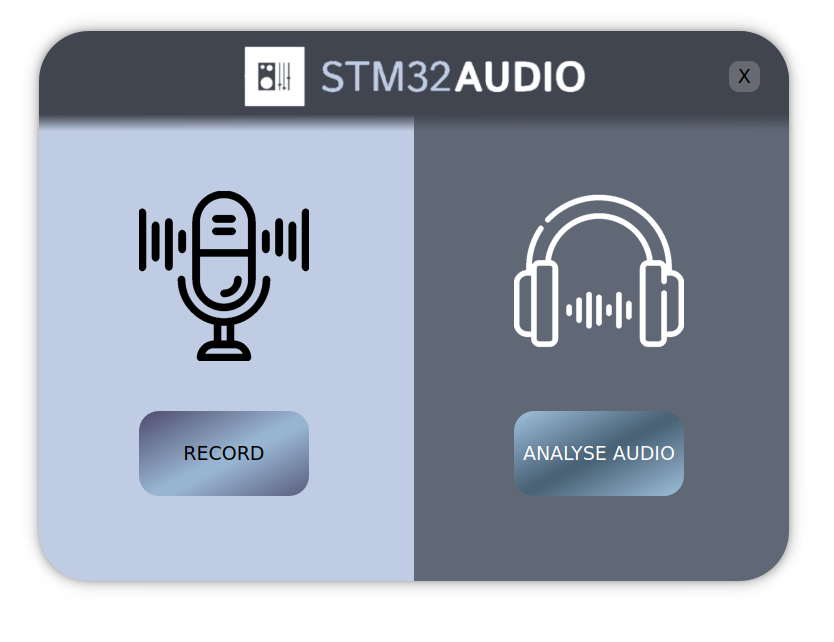
\includegraphics[width=\linewidth]{imgs/intro_form}
	\caption{Uvodni izbornik}
	\label{fig:intro_form}
\end{figure}


U sučelju za postavljanje parametara snimanja korisnik postavlja trajanje snimanja zvuka koje je ograničeno na minimalno 1 sekundu te maksimalno 24 sata. Korisnik također može odabrati opciju pohrane zvučnog zapisa na računa, kao i trenutnu reprodukciju snimanog zvuka na računalu. Trenutna reprodukcija zvuka nije preporučljiva ako se mikrokontroler i računalo nalaze u istoj prostoriji jer može doći do mikrofonije, koja se događa kada mikrofon prima zvuk iz uređaja za reprodukciju zvuka. Klikom na gumb \textit{Start recording} otvara se novo sučelje u kojem se pokreće Bluetooth skeniranje i snimanje zvuka.

\begin{figure}[ht]
	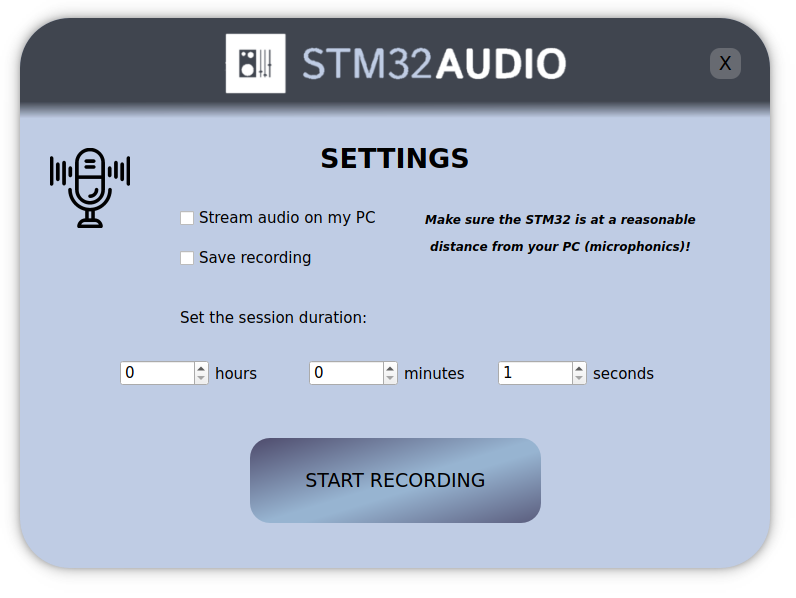
\includegraphics[width=\linewidth]{imgs/params_form}
	\caption{Sučelje za podešavanje parametara}
	\label{fig:params_form}
\end{figure}

Gumb \textit{Start} pokreće Bluetooth skeniranje uređaja na računalu. Ako nije pronađen uređaj s kojim se računalo može upariti, sustav obavještava korisnika te omogućuje ponovno skeniranje uređaja. 

Nakon uparivanja s pronađenim uređajem, pokreće se snimanje zvuka na mikrokontroleru. Korisničko sučelje ispisuje na ekranu prethodno postavljene parametre snimanja i preostalo vrijeme do kraja snimanja. Na završetku primljeni se zvučni zapis pohranjuje obliku \textit{RAW} datoteke, koja se zatim sprema u direktorij \textit{audioDumps}. Svaki zvučni zapis u svom nazivu sadrži vremensku oznaku početka snimanja. 

Snimanje je moguće pokrenuti ponovno pritiskom na gumb \textit{Start}, ali s ranije definiranim parametrima.

\vspace*{3\baselineskip}
 
%%
%mini slikice%
\begin{figure}[ht]
	\begin{minipage}[t]{0.4\textwidth}
		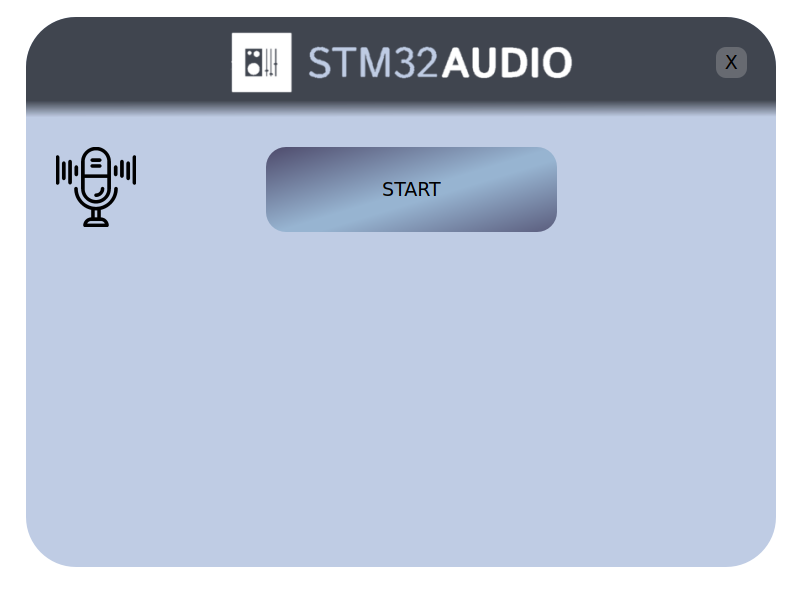
\includegraphics[width=\linewidth]{imgs/recording_form}
		\caption{Prije pokretanja snimanja}
		\label{fig:recording_form}
	\end{minipage}
	\hspace*{\fill}
	\begin{minipage}[t]{0.4\textwidth}
		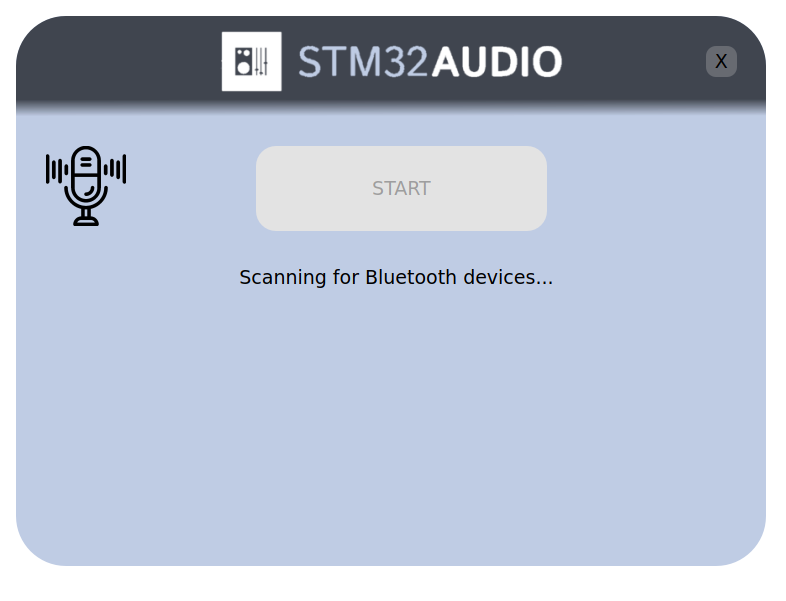
\includegraphics[width=\linewidth]{imgs/recording_form_2}
		\caption{Skeniranje uređaja}
		\label{fig:recording_form_2}
	\end{minipage}
\end{figure}

\begin{figure}[ht]
	\begin{minipage}[t]{0.4\textwidth}
	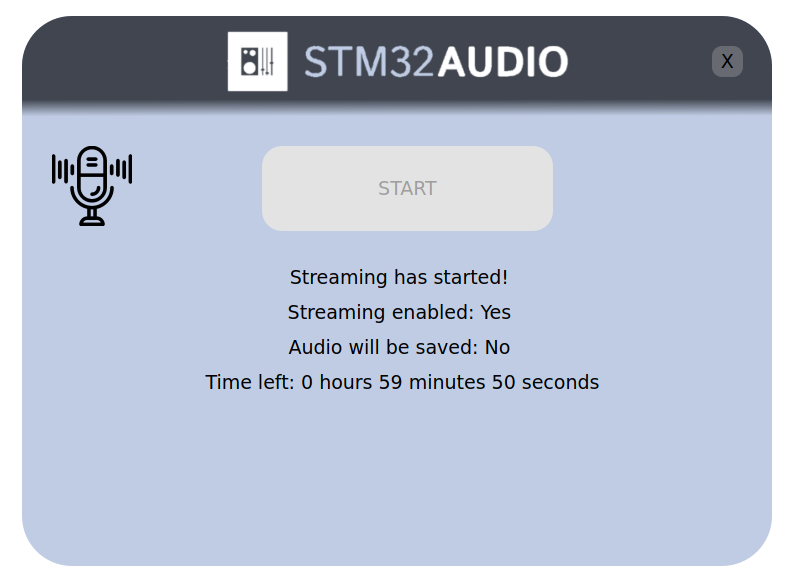
\includegraphics[width=\linewidth]{imgs/recording_form_3}
	\caption{Snimanje zvuka}
	\label{fig:recording_form_3}
	\end{minipage}
	\hspace*{\fill}
	\begin{minipage}[t]{0.4\textwidth}
		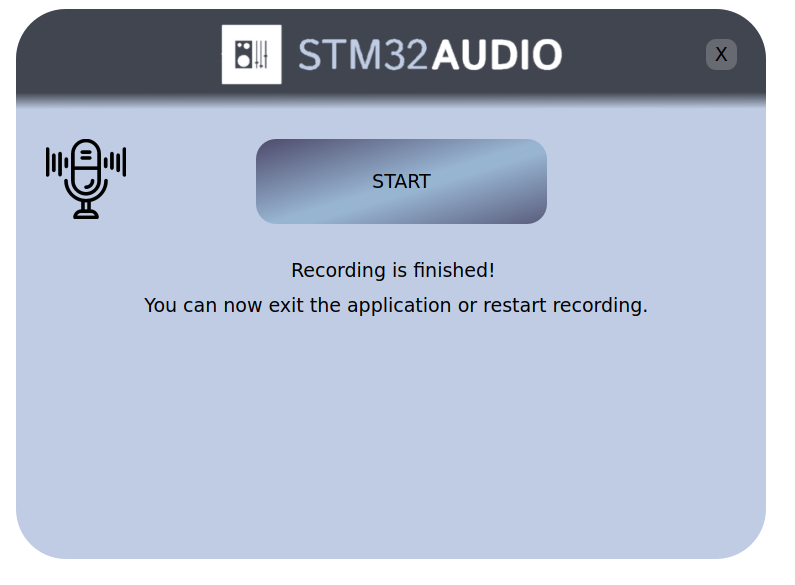
\includegraphics[width=\linewidth]{imgs/recording_form_4}
		\caption{Završetak snimanja}
		\label{fig:recording_form_4}
	\end{minipage}
\end{figure}
%end mini slikice%
%%


Glavni prozor i ostali elementi korisničkog sučelja konfiguriraju se u klasi \textit{Ui\_Form}, odnosno u njezinoj funkciji \lstinline|setupUi|, koja kao parametar prima \textit{Form} objekt. Taj objekt nasljeđuje dvije klase - \textit{QWidget}, kao glavni prozor s grafičkim komponentama, i samu \textit{Ui\_Form} klasu, kako bi se glavni prozor mogao pomicati povlačenjem miša. 

\begin{lstlisting}[caption={Definicija klase \textit{Form} i njezin konstruktor}, language=Python]
	class Form(QtWidgets.QWidget, Ui_Form):
		def __init__(self, parent=None):
		super(Form, self).__init__(parent)
		self.setupUi(self)
		self.setMouseTracking(True)
\end{lstlisting}

Također, definiraju se dva objekta za praćenje vremena:
\begin{enumerate}
	\item \textit{QTimer}: pokreće se u trenutku početka snimanja zvuka i trajanje mu je određeno na prethodnom sučelju. Služi za prikaz preostalog vremena i signalima je povezan s metodom \lstinline|finished| koja ispisuje poruku o završetku snimanja.
	\item \textit{QBasicTimer}: služi za osvježavanje grafičkog prikaza svake sekunde. Zaustavlja se istekom vremena postavljenog objektom \textit{QTimer}, odnosno aktiviranjem metode \lstinline|finished|. Povezan je signalima s funkcijom \lstinline|timerEvent| koja poziva metodu \lstinline|update_gui| za ponovno iscrtavanje sučelja.
\end{enumerate}

Za pokretanje korisničkog sučelja potrebno je najprije napraviti instancu objekta \textit{QApplication} koja upravlja tijekom kontrole GUI aplikacije i glavnim postavkama. \textit{QApplication} sadrži glavnu petlju događaja, gdje se obrađuju i šalju svi događaji iz prozorskog sustava i drugih izvora. Također upravlja inicijalizacijom, finalizacijom aplikacije i pruža upravljanje sesijom. Osim toga, \textit{QApplication} obrađuje većinu postavki za cijeli sustav i aplikaciju. Za bilo koju GUI aplikaciju koja koristi \textit{Qt}, postoji točno jedan \textit{QApplication} objekt, bez obzira na broj prozora. 

Metoda \lstinline|exec_| pokreće glavnu petlju događaja i čeka dok se ne pozove \lstinline|exit| funkcija. Potrebno je pozvati ovu funkciju za početak rukovanja događajima. Glavna petlja događaja prima događaje iz prozorskog sustava i šalje ih widgetima aplikacije. Potrebno je pozvati ovu funkciju za početak rukovanja događajima. Glavna petlja događaja prima događaje iz prozorskog sustava i šalje ih elementima  aplikacije.

\begin{lstlisting}[caption={Naredbe za pokretanje korisničkog sučelja}, language=Python]
	import sys
	app = QtWidgets.QApplication(sys.argv)
	w = Form()
	w.show()
	sys.exit(app.exec_())
\end{lstlisting}


\section{Višedretvenost sučelja i programske potpore}

PyQt aplikacije s grafičkim korisničkim sučeljem imaju glavnu dretvu koja pokreće glavnu petlju događaja i GUI. Pokrene li se dugotrajni zadatak u ovoj dretvi, GUI će se zamrznuti sve dok se zadatak ne izvrši. Za to vrijeme korisnik ne može komunicirati s aplikacijom, niti se prikaz sučelja može mijenjati tijekom izvođenja zadatka. Stoga je izvođenje dugotrajnih zadataka potrebno odvojiti od rada korisničkog sučelja.

U ovoj aplikaciji prikaz sučelja i programska potpora koja obavlja povezivanje Bluetoothom i snimanje zvuka izvršavaju se paralelno, stoga ih je potrebno izvoditi simultano u dvjema dretvama koje međusobno komuniciraju. Iako Python u svojoj biblioteci nudi module za rad s dretvama, u ovoj je aplikaciji korištena klasa \textit{QtThread} koja se nalazi u okviru PyQt radi povezivanja rada dretvi sa signalima i događajima.

PyQt aplikacije imaju dvije vrste dretvi:
\begin{itemize}
	\item Glavna dretva
	\item \textit{Worker} dretve
\end{itemize}

Glavna dretva aplikacije uvijek postoji te se još naziva i GUI dretva. S druge strane, \textit{worker} dretve ovise o potrebama aplikacije i može ih biti proizvoljno mnogo. One su sekundarne dretve koje se mogu koristiti za rasterećivanje glavnog programa i odvajanje dugotrajnih zadataka iz glavne dretve, čime se sprječava smrzavanje korisničkog sučelja. 

Svaki \textit{QThread} objekt upravlja jednom dretvom unutar programa i njihov rad započinje metodom \lstinline|run|. Ta metoda pokreće petlju događaja unutar dretve pozivanjem funkcije \lstinline|exec|. Važno je naglasiti da \textit{QThread} objekt nije dretva sam po sebi, nego je omotač oko dretve operacijskog sustava. Prava dretva kreira se pozivom funkcije \lstinline|QThread.start()|.

\textit{Worker} klasa nasljeđuje \textit{QObject} klasu i u nju je smještena programska potpora za povezivanje računala s mikrokontrolerom. Također su definirana tri signala koja komuniciraju s glavnom dretvom - jedan koji signalizira kraj izvođenja procesa, drugi za ažuriranje tekstualnog prikaza, i treći koji signalizira početak snimanja zvuka. Svaki od signala pozivom metode \lstinline|emit| emitira signal glavnoj petlji o vlastitoj promjeni. 

\begin{lstlisting}[caption={\textit{Worker} klasa}, language=Python]
	class Worker(QObject):
		# Class for running BLE 
		finished = pyqtSignal()
		textlabel = pyqtSignal(str)
		stream = pyqtSignal()
	
		def run(self):
			self.textlabel.emit("Scanning for devices...")
			# ... code for BLE connection ... 
			return
\end{lstlisting}

Isječak koda 4.4 prikazuje princip povezivanja glavne, GUI dretve s \textit{worker} dretvom koja povezuje rad mikrokontrolera i računala.

Za početak je potrebno stvoriti instance \textit{QThread} i \textit{Worker} klase. Nakon toga, funkcijom \lstinline|moveToThread| funkcionalnost \textit{Worker} klase prebacuje se u \textit{QThread} objekt koji će se izvršavati neovisno o GUI dretvi. Zatim je potrebno povezati signale dretve s funkcijama koje će se izvršiti pri emisiji signala. Naposljetku, izvršavanje dretve započinje pokretanjem metode \lstinline|start| nad \textit{QThread} objektom, što ujedno i emitira \lstinline|started| signal koji je povezan s metodom \lstinline|run| objekta \textit{Worker}. Time je započet rad te klase u odvojenoj dretvi bez ikakve ovisnosti o glavnoj dretvi s korisničkim sučeljem.

\begin{lstlisting}[caption={Povezivanje glavne dretve s \textit{worker} dretvom}, language=Python]
	# Step 1: Create a QThread object
	self.thread = QThread()
	# Step 2: Create a worker object
	self.worker = Worker()
	# Step 3: Move worker to the thread
	self.worker.moveToThread(self.thread)
	# Step 4: Connect signals and slots
	self.thread.started.connect(self.worker.run)
	self.worker.finished.connect(self.thread.quit)
	...
	# Step 5: Start the thread
	self.thread.start()
\end{lstlisting}


\eject